\chapter{Multi-channel APR system details}\label{ap:MultiAPRsystem}

\ifpdf
    \graphicspath{{Appendices/AppendixMultiAPRsystem/Photos/}{Appendices/AppendixMultiAPRsystem/Figs/}}
\else
\fi

As seen in Figure~\ref{fig:MultiAPRsystem.pdf}, on page~\pageref{fig:MultiAPRsystem.pdf}, and Figure~\ref{fig:wholesystem} the multi-channel \gls{apr} system was constructed of a block of medium-density fibreboard wood $30.6 \times 24.3 \times 1.8$ cm (l$\times$w$\times$d), with 6 1cm diameter 2 cm deep holes drilled into it from the back. On the front of the surface a grid was marked out and 9 points were marked out. These 9 spots can be seen as squares drawn in pencil on Figure~\ref{fig:frontfacesurface}.
\begin{figure}[b!]
\centering
\begin{subfigure}{.5\textwidth}
  \centering
  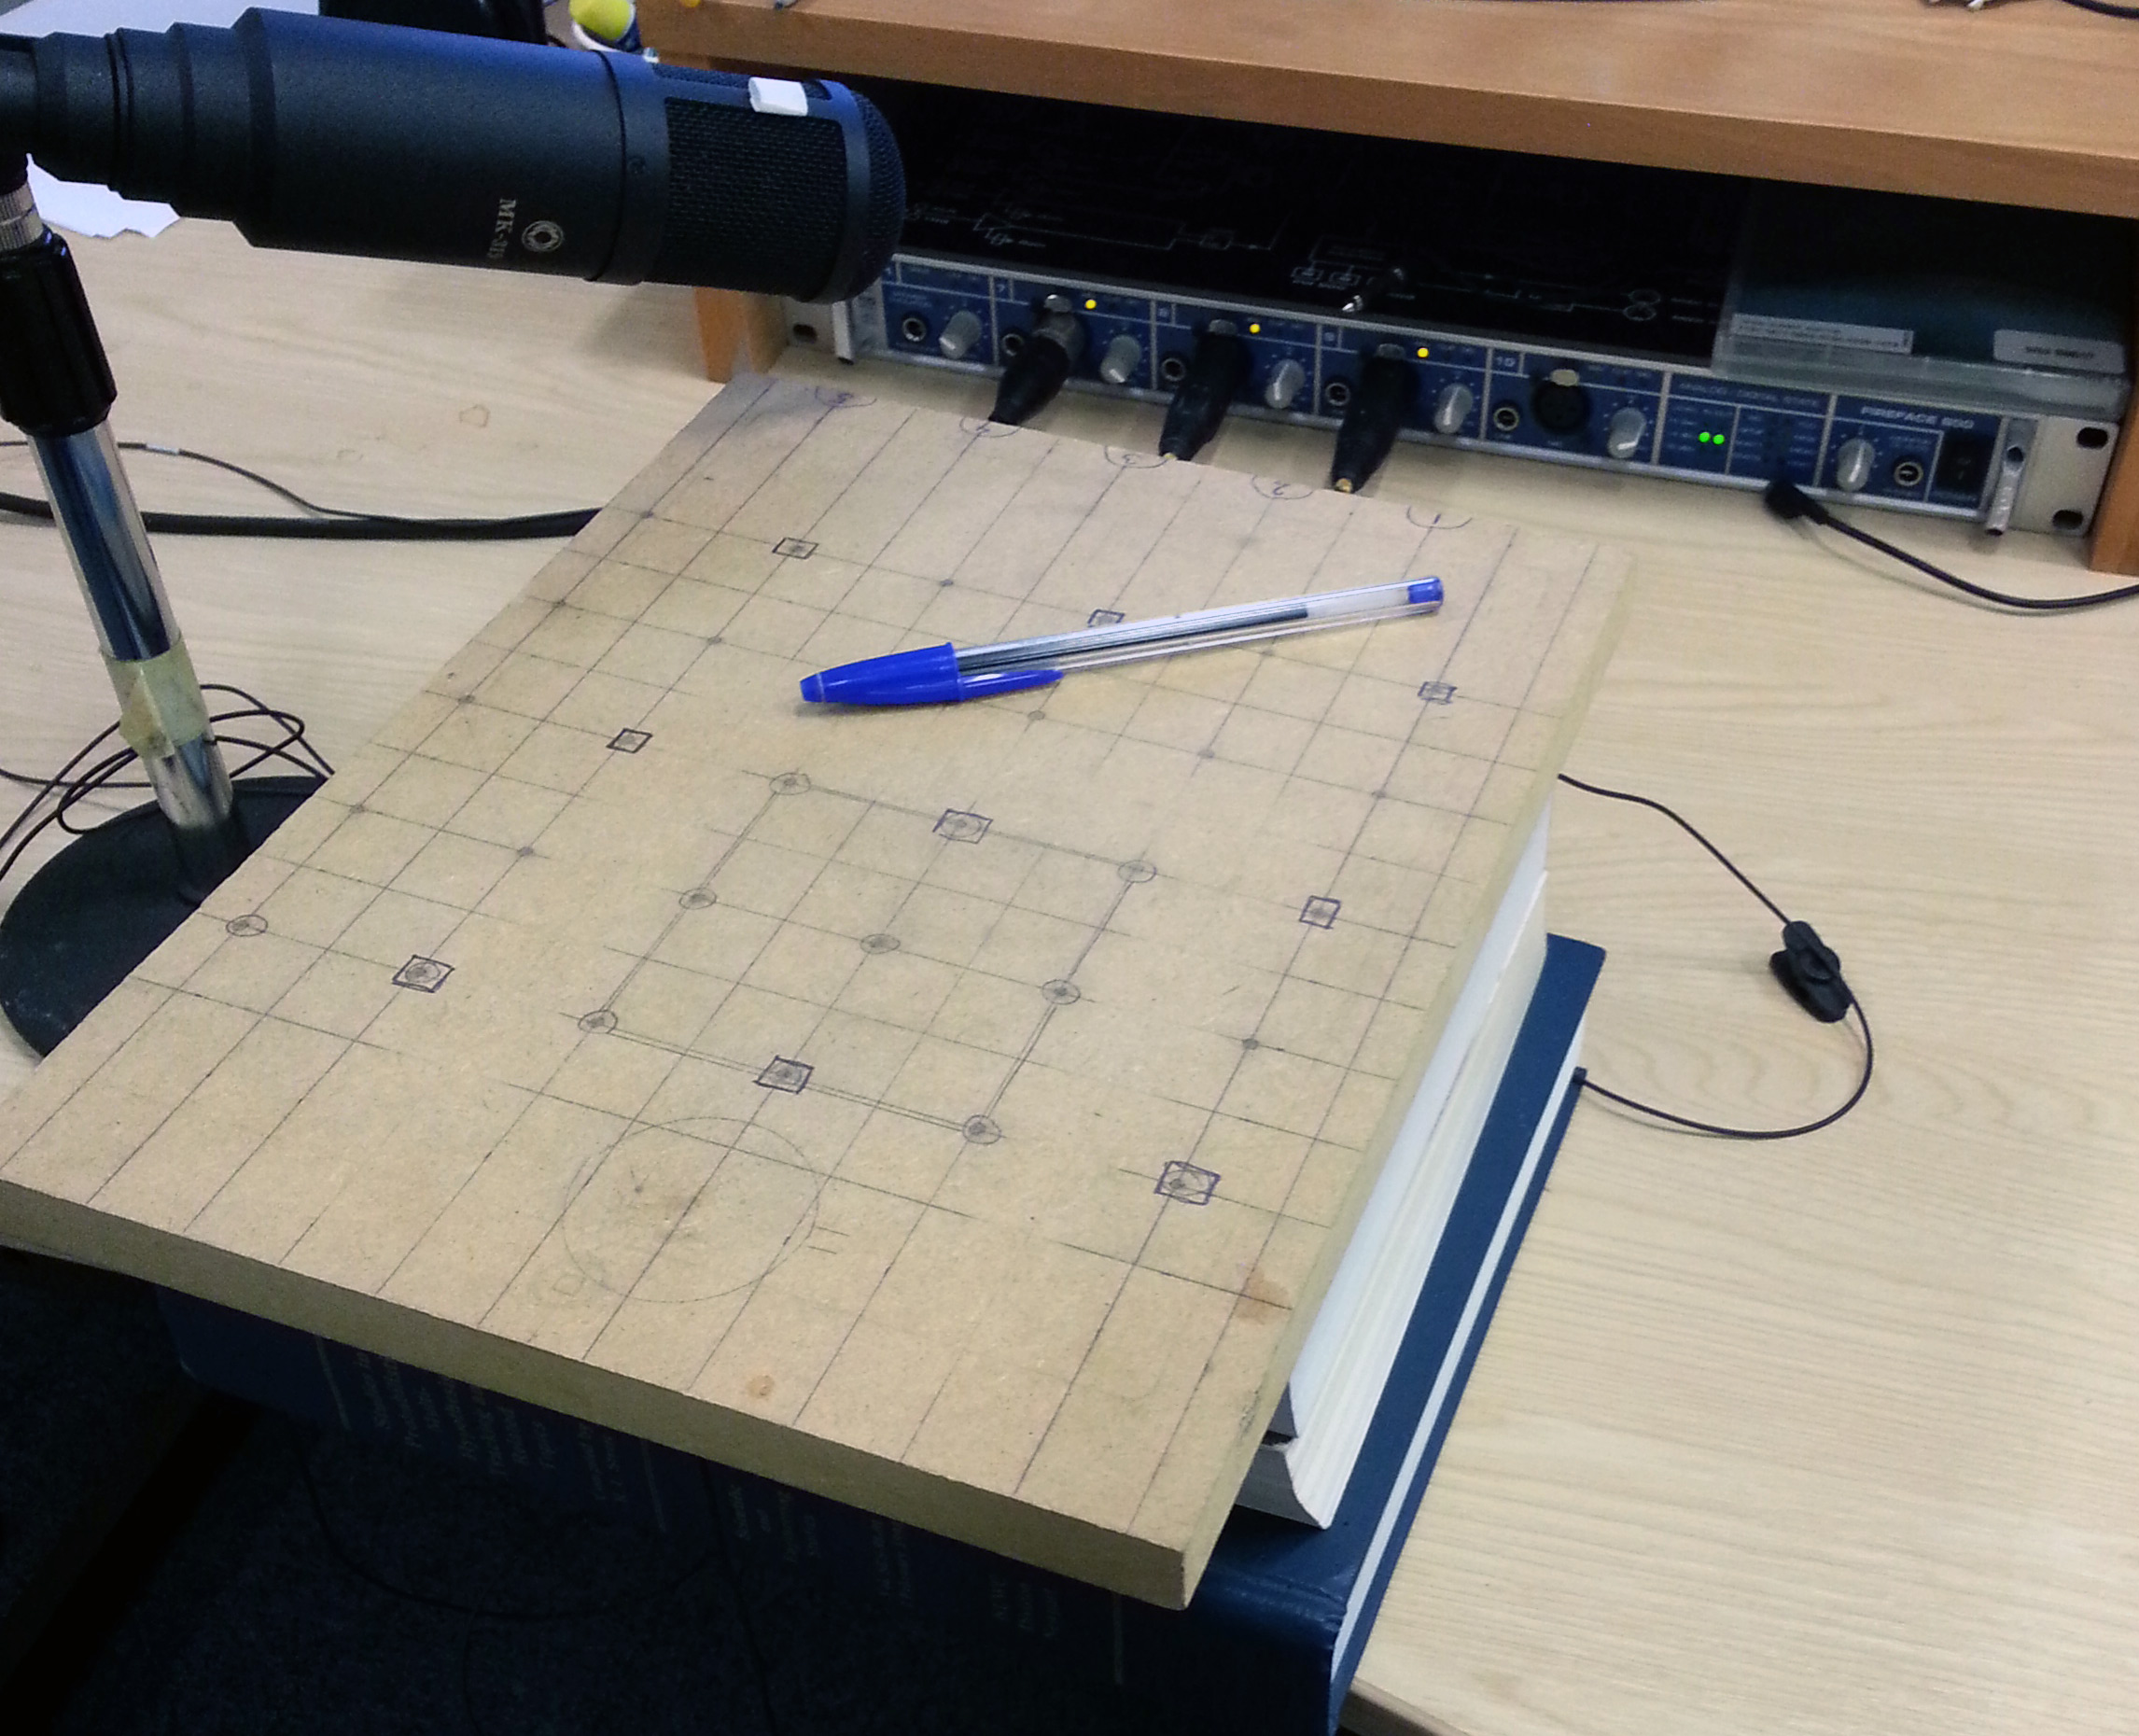
\includegraphics[width=7cm]{wholesystem}
  \caption{The entire multi-channel \gls{apr} system setup.}
  \label{fig:wholesystem}
\end{subfigure}%
\begin{subfigure}{.5\textwidth}
  \centering
  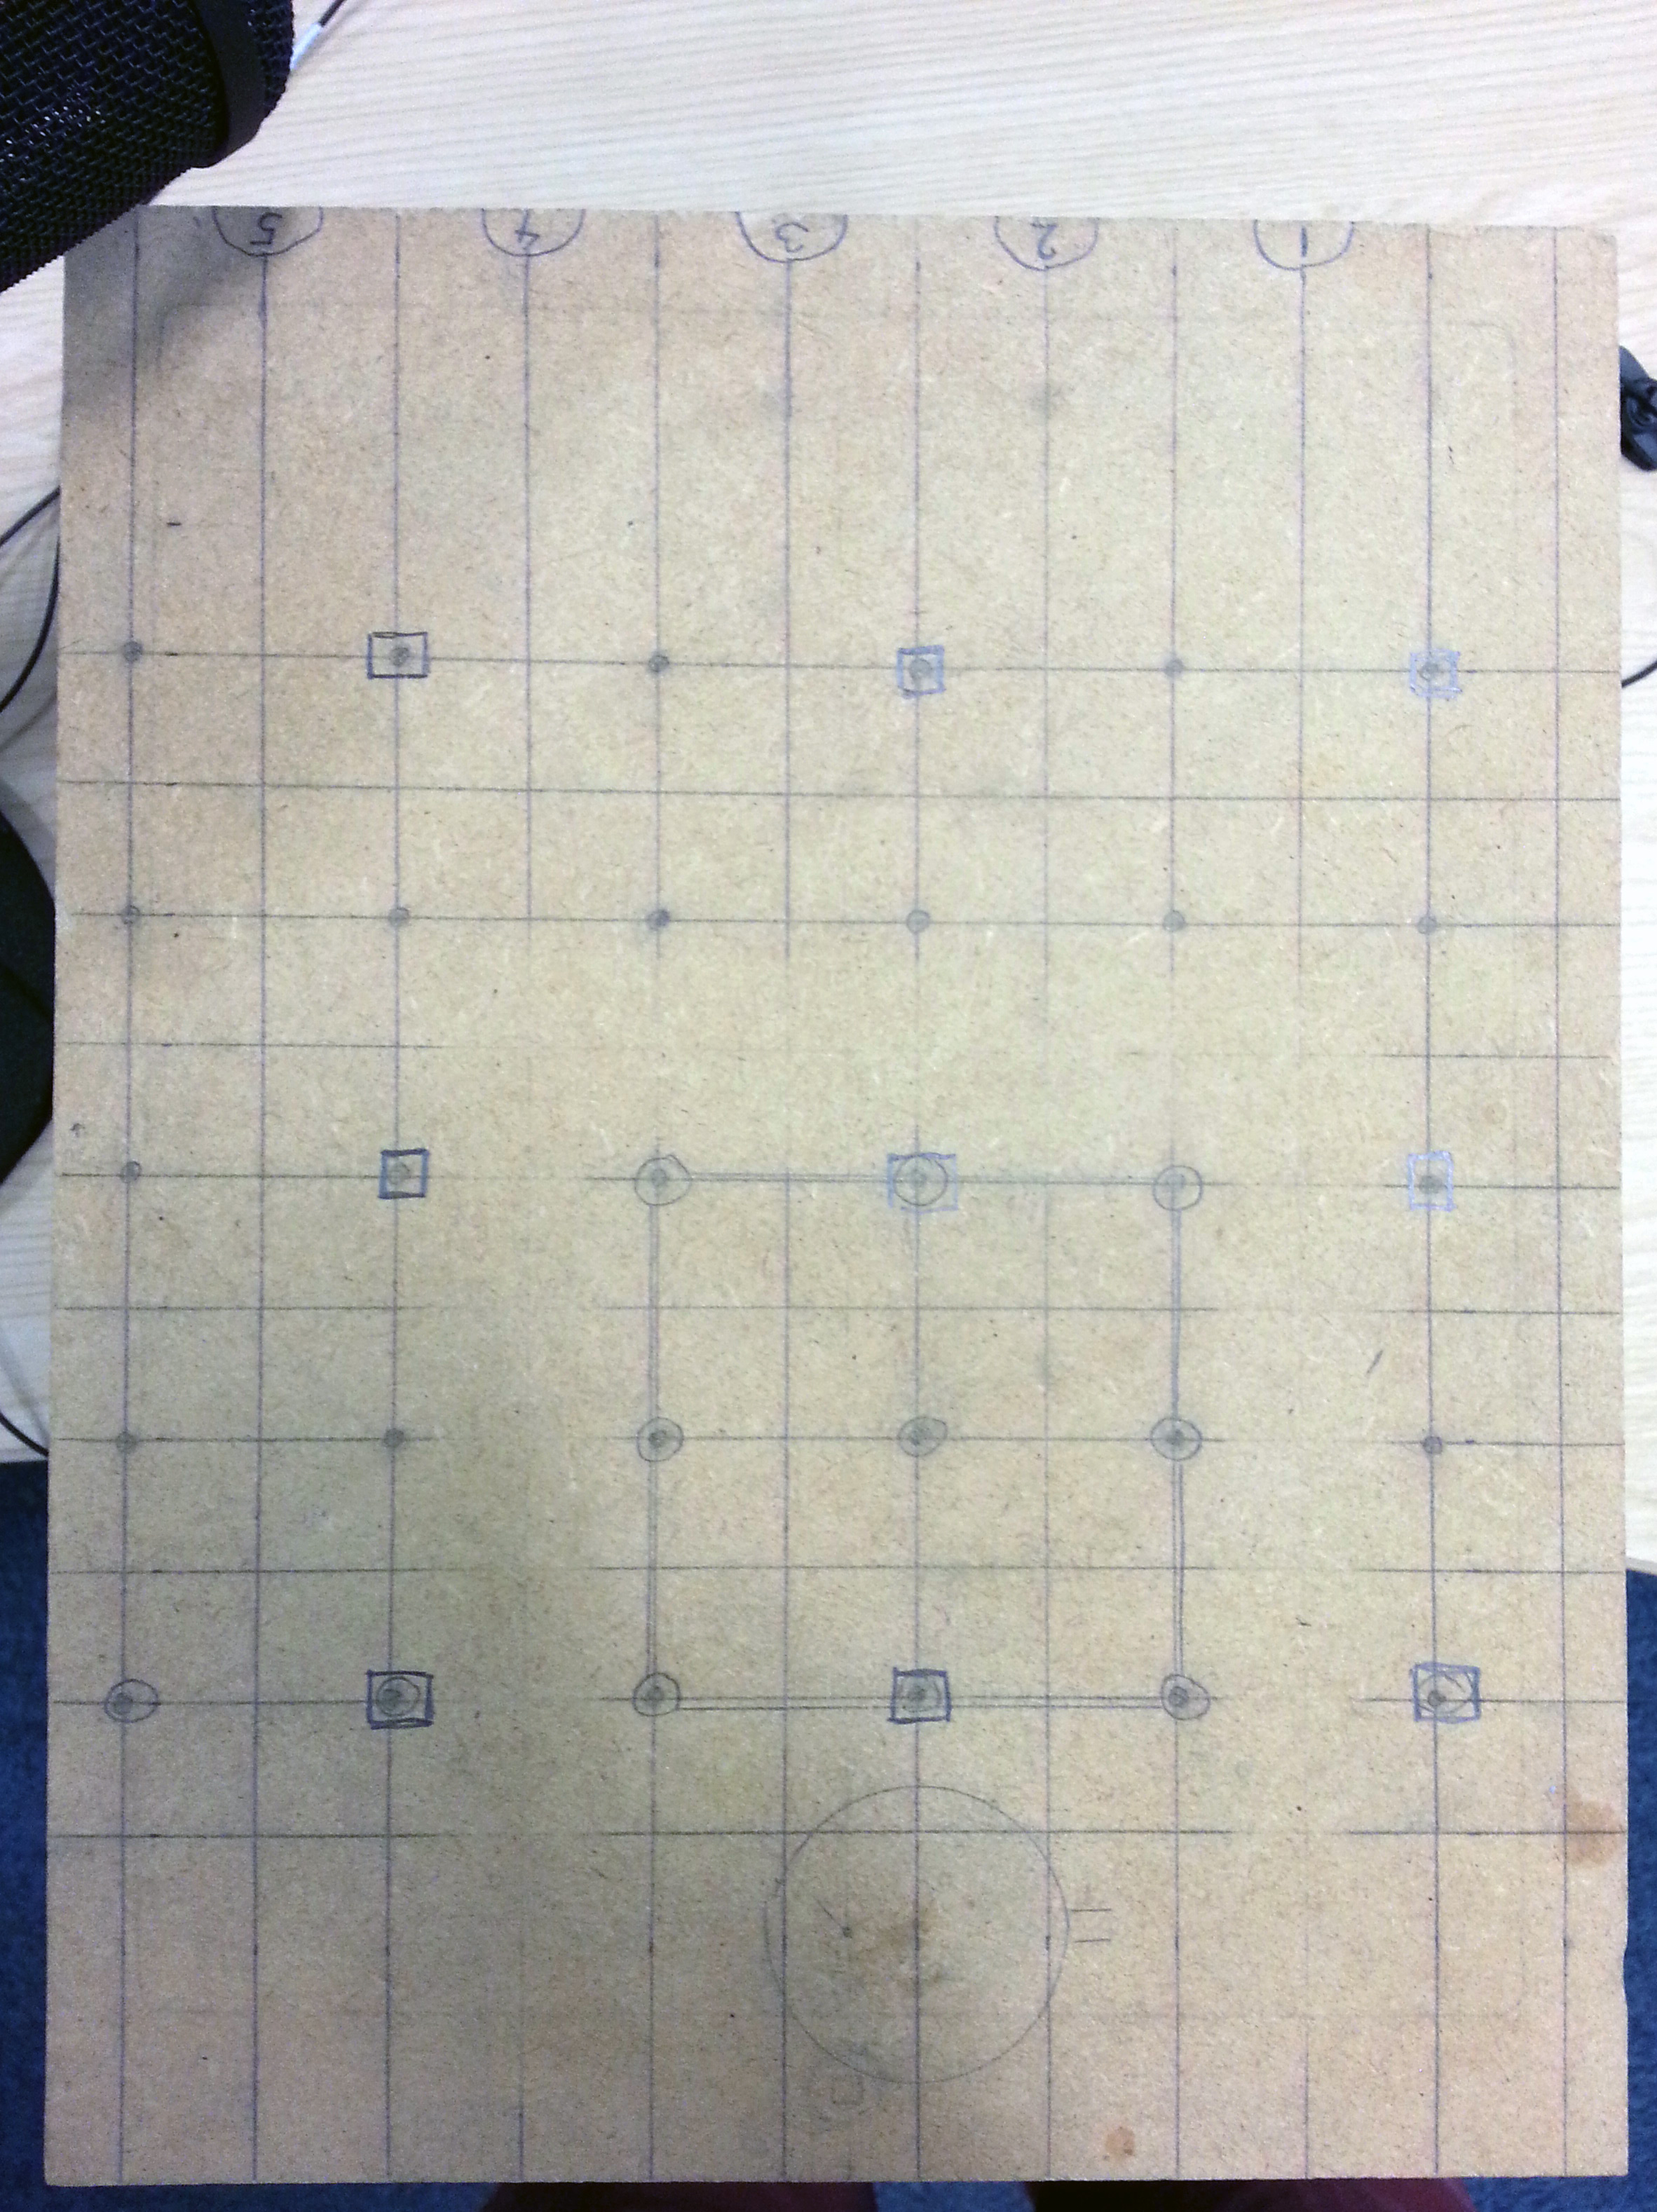
\includegraphics[width=5cm]{surface}
  \caption{The front face of the surface.}
  \label{fig:frontfacesurface}
\end{subfigure}
\caption{The multi-channel system setup}
\label{fig:multiAPRsystemwhole}
\end{figure}

\begin{figure}[t!]
\begin{minipage}[b]{1.0\linewidth}
  \centering
  \centerline{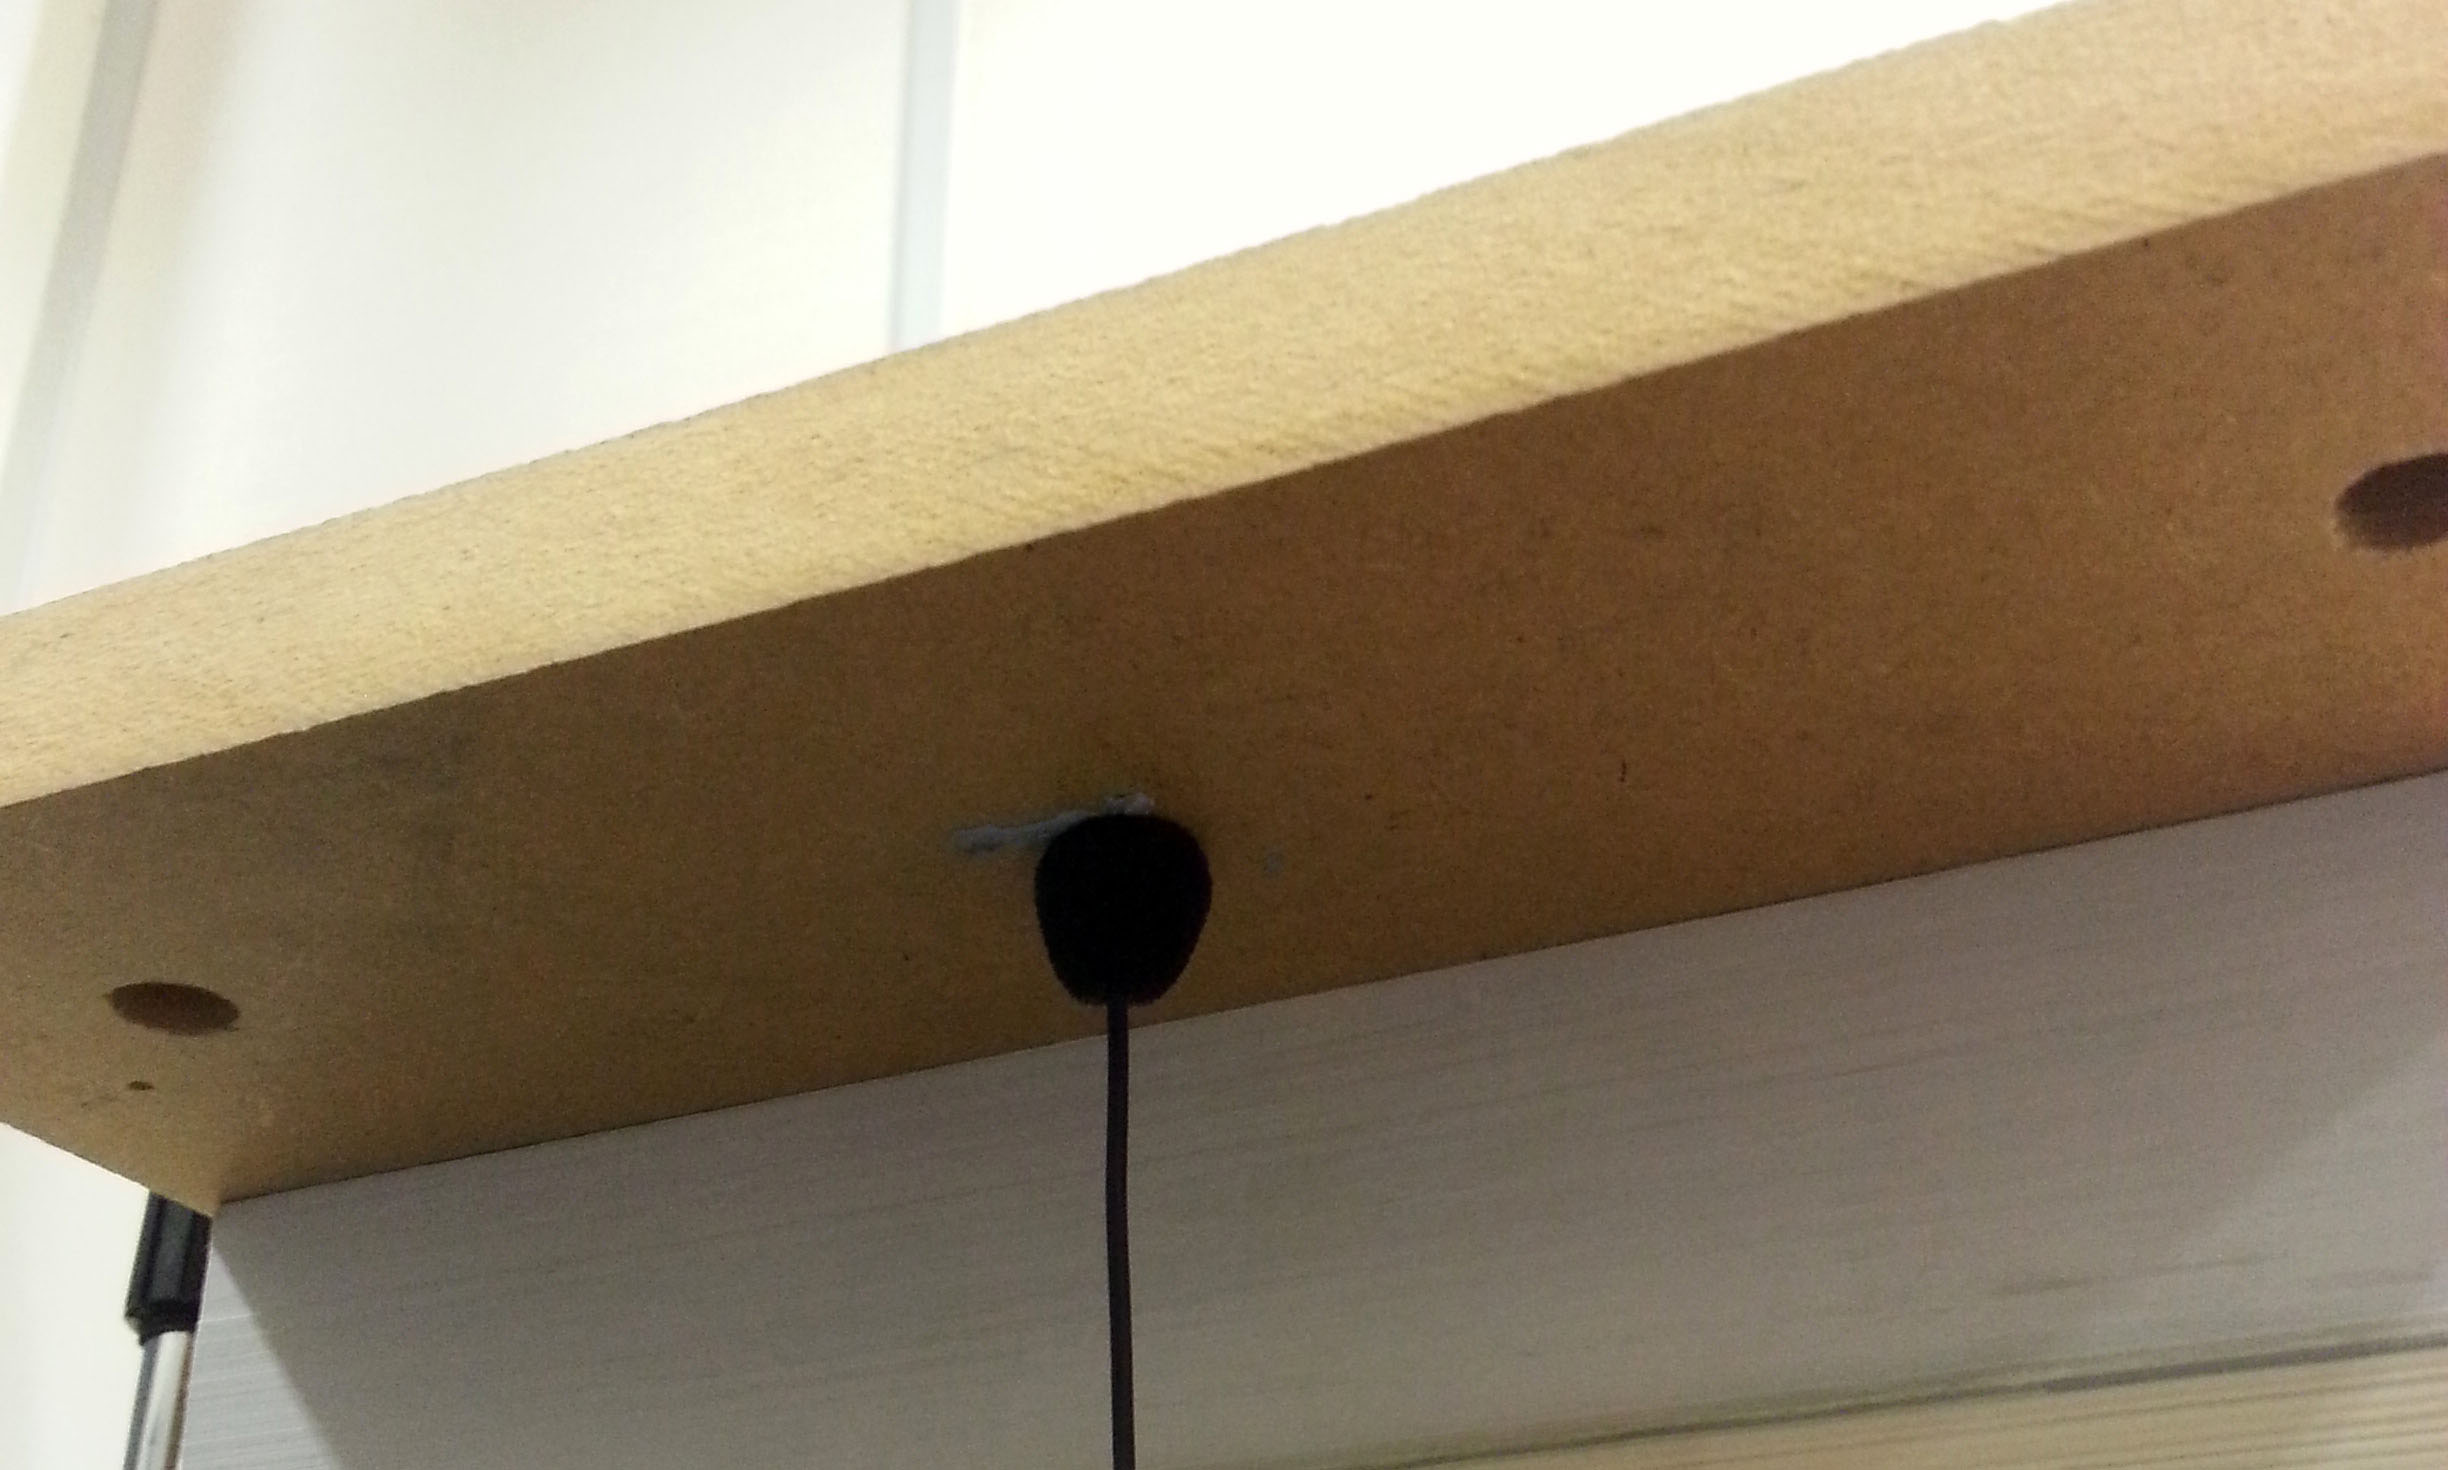
\includegraphics[width=10cm]{mic2}}%10
  %\vspace{.5cm}
  \centerline{(a) Microphone 2}\medskip
\end{minipage}
\begin{minipage}[b]{1.0\linewidth}
  \centering
  \centerline{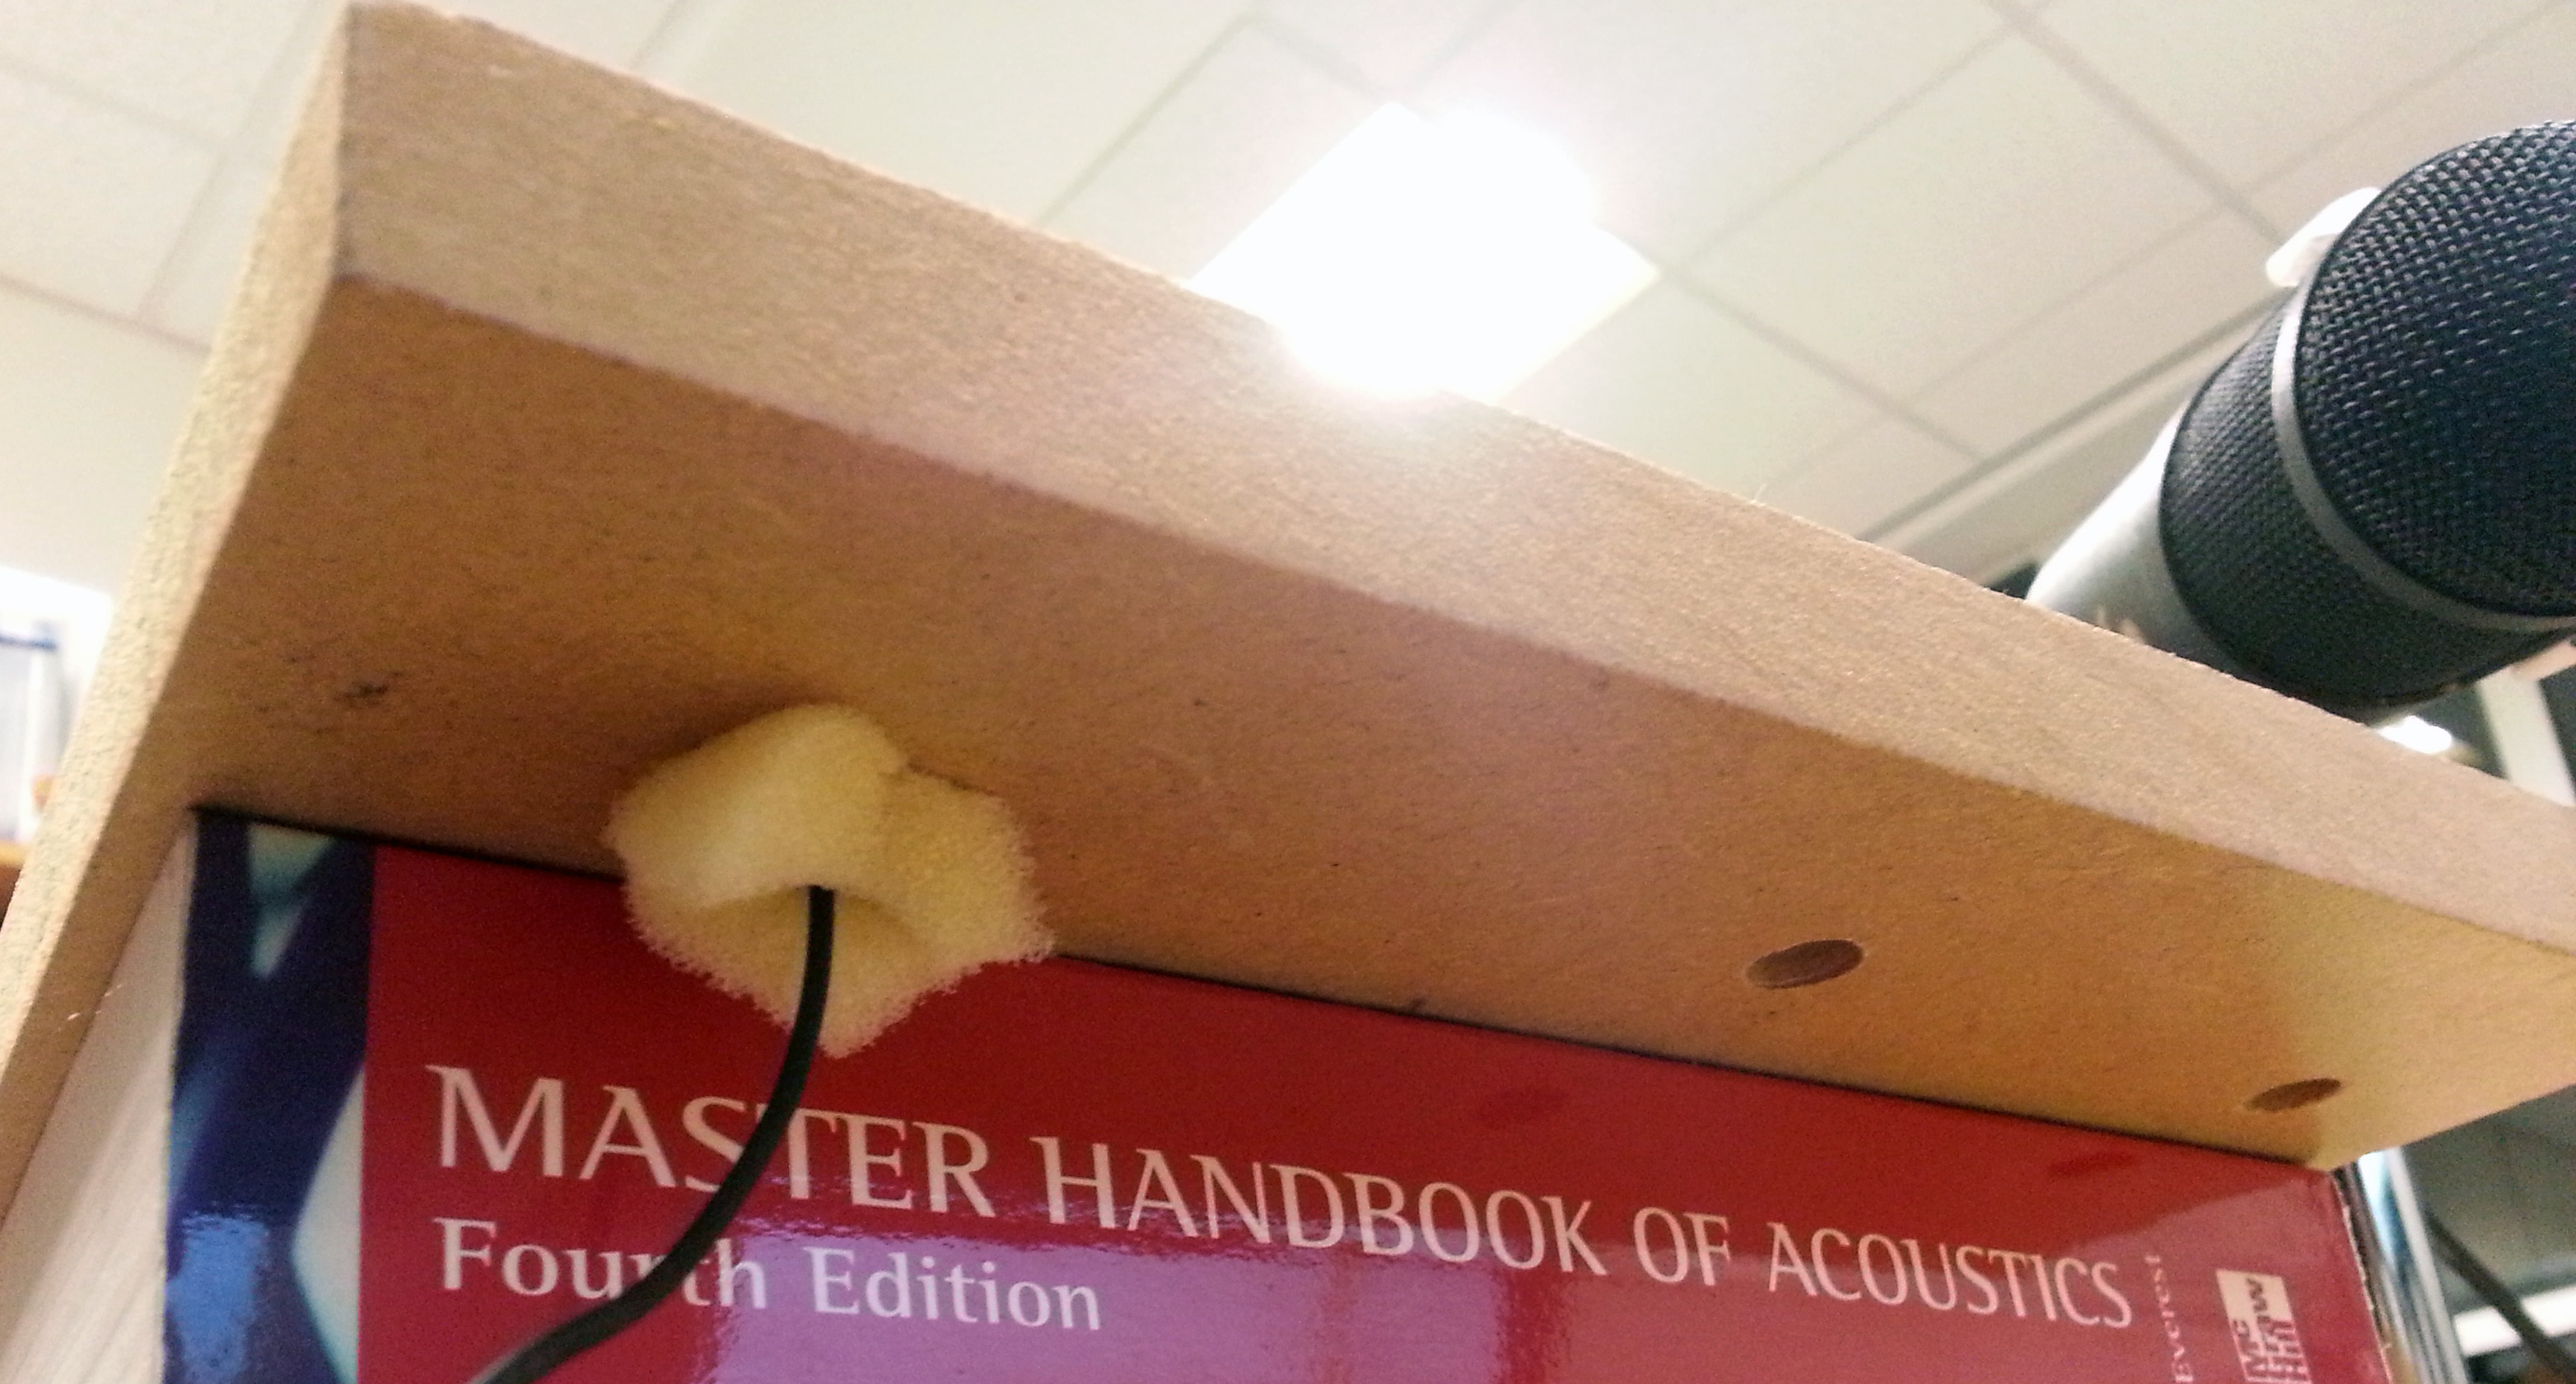
\includegraphics[width=10cm]{mic3}}%10
  %\begin{picture}(0,0)
%\put(-120,382){(a)}
%\put(-120,195){(b)}
%\end{picture}
 %\vspace{1.5cm}
  \centerline{(b) Microphone 3}\medskip
\end{minipage}
\caption{Microphones 2 and 3 embedded in the back of the surface.}
\label{fig:mic23}
\end{figure}


Microphone 1, seen in Figures~\ref{fig:mic1} and \ref{fig:wholesystem}, was an Oktava MK-319 large diaphragm condenser microphone. This microphone was positioned slightly above and outside the edge of the surface. Figure~\ref{fig:mic23}(a) and (b) shows microphones 2 and 3, respectively. These were DPA 4060 miniature condenser microphones. All microphones were omnidirectional with no padding or equalising applied. As noted in Figure~\ref{fig:mic23}(a) and (b) microphones 2 and 3 were positioned into the drilled holes in the back of the surface and held in place with low density foam.


\begin{figure}
\centering
\begin{subfigure}{.5\textwidth}
  \centering
  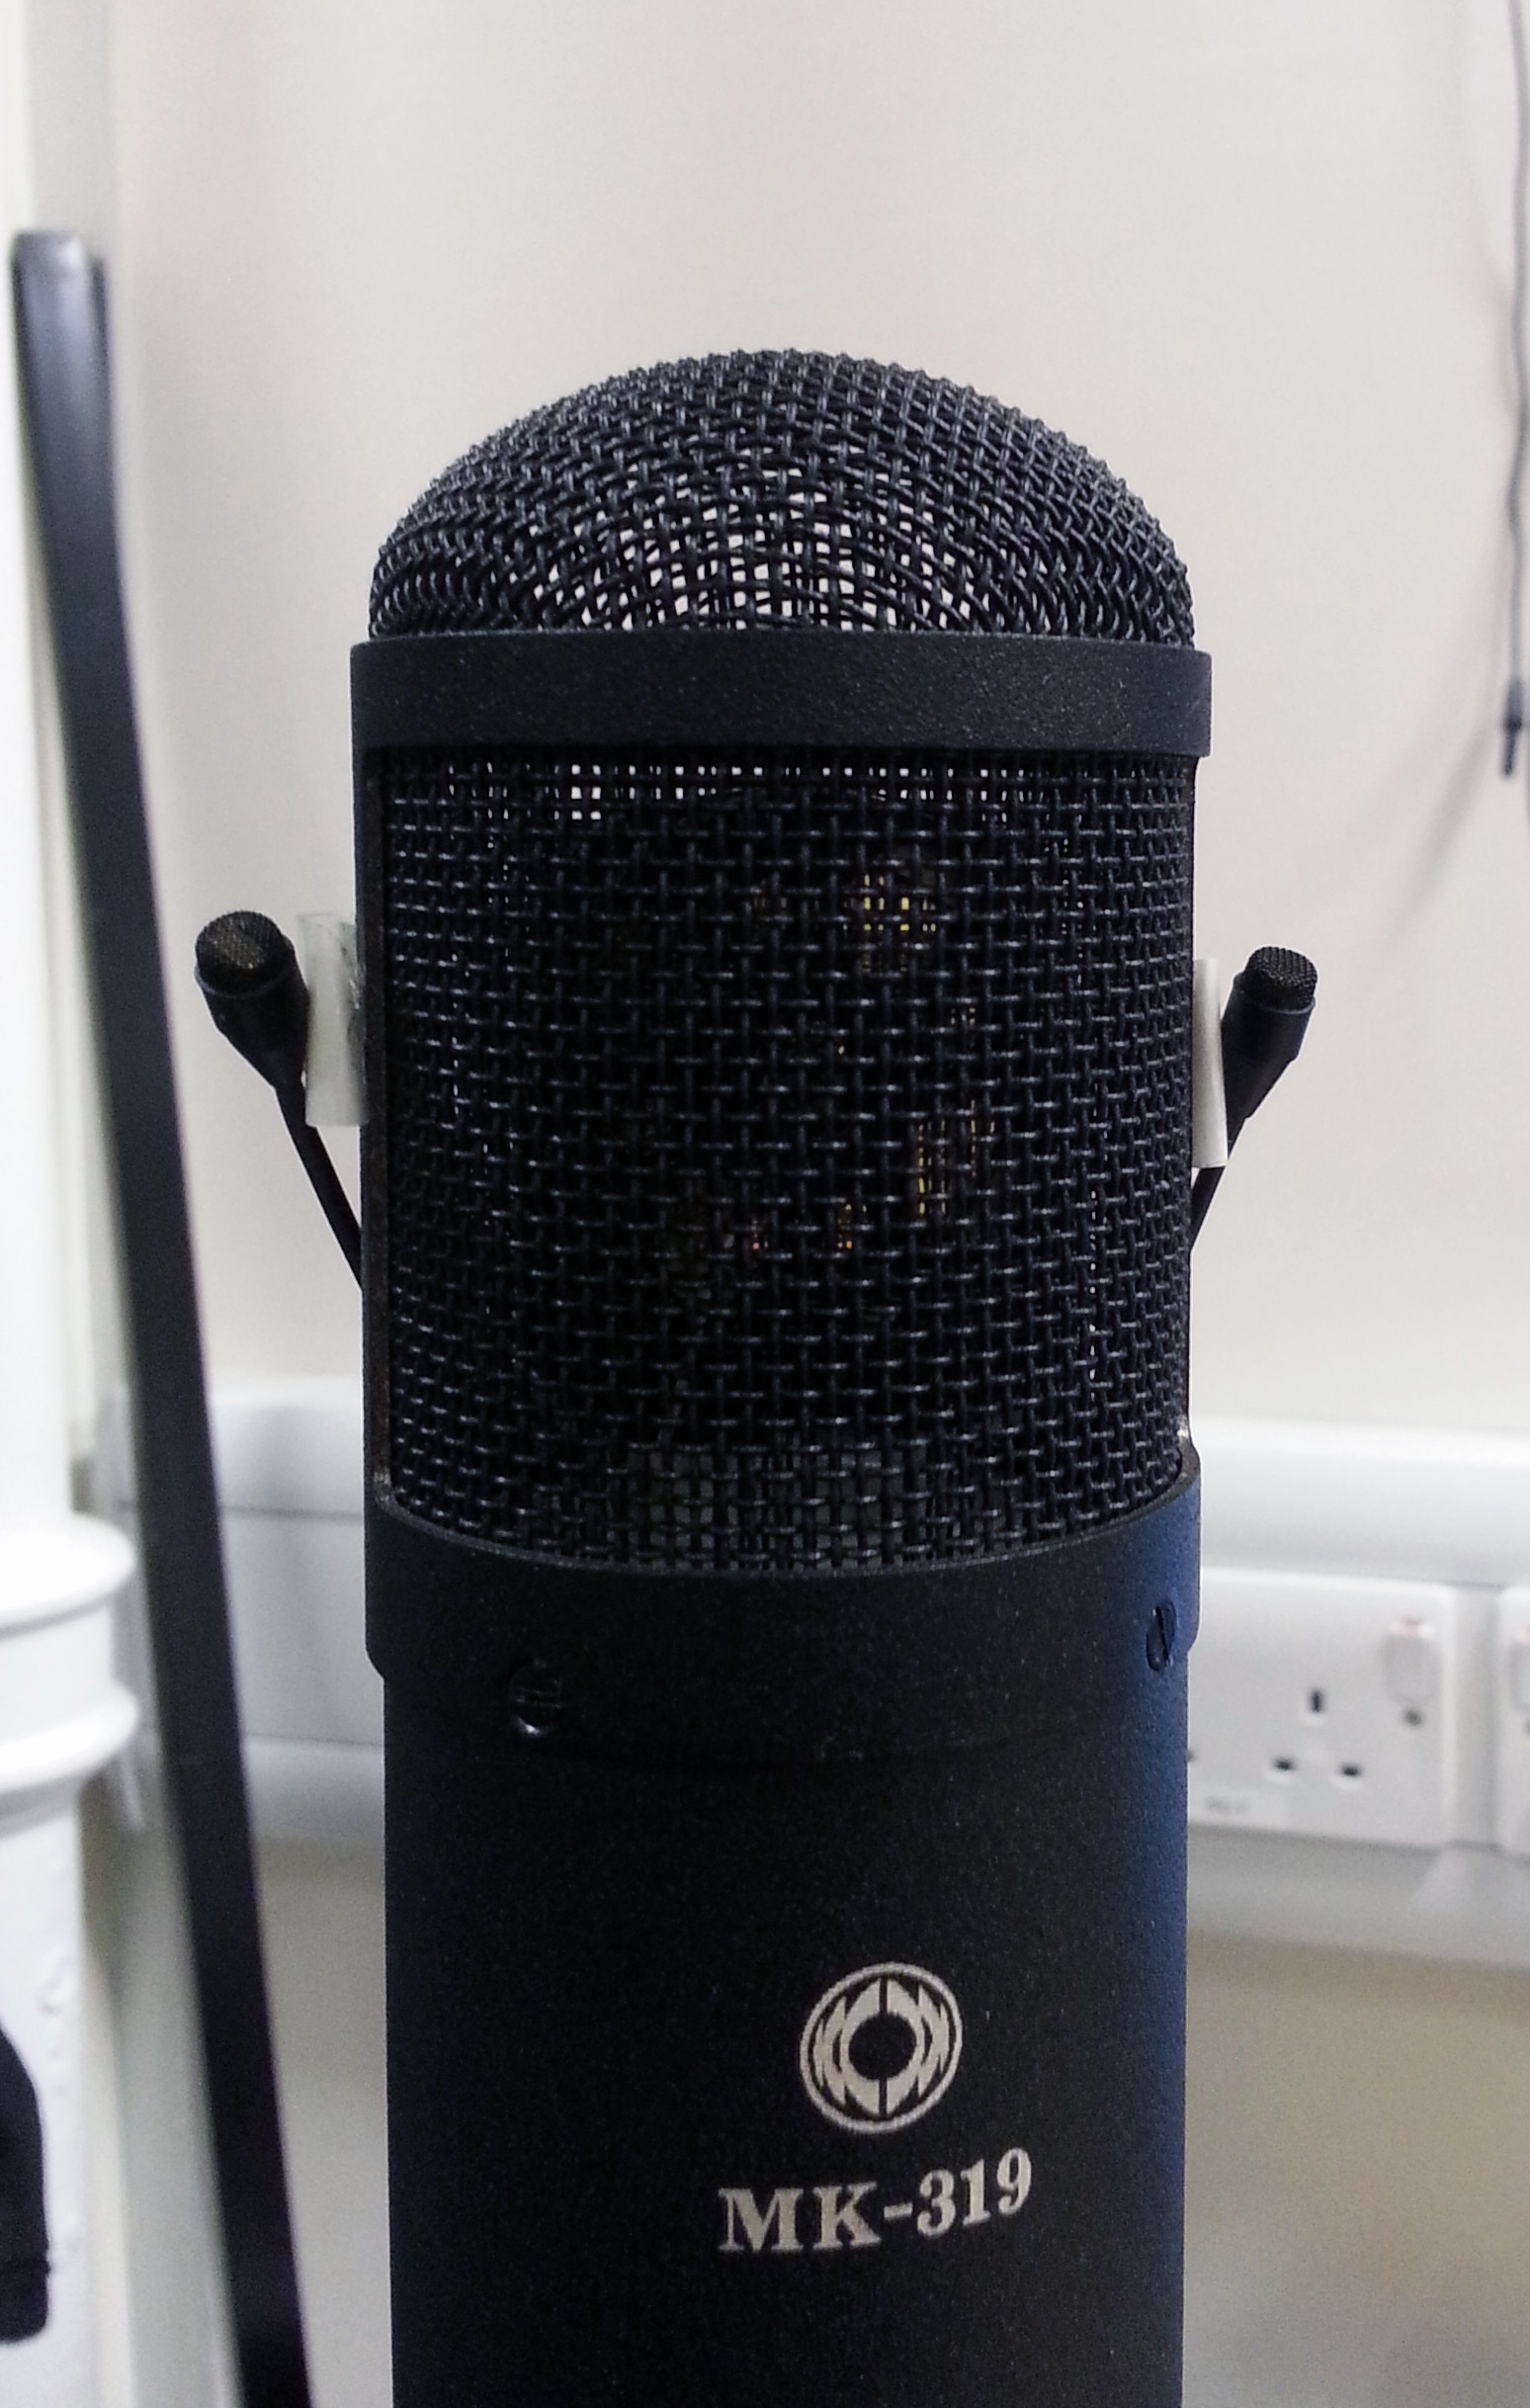
\includegraphics[width=4cm]{micsAlign}%4
  \caption{All microphones used aligned spatially.}
  \label{fig:micsaligned}
\end{subfigure}%
\begin{subfigure}{.5\textwidth}
  \centering
  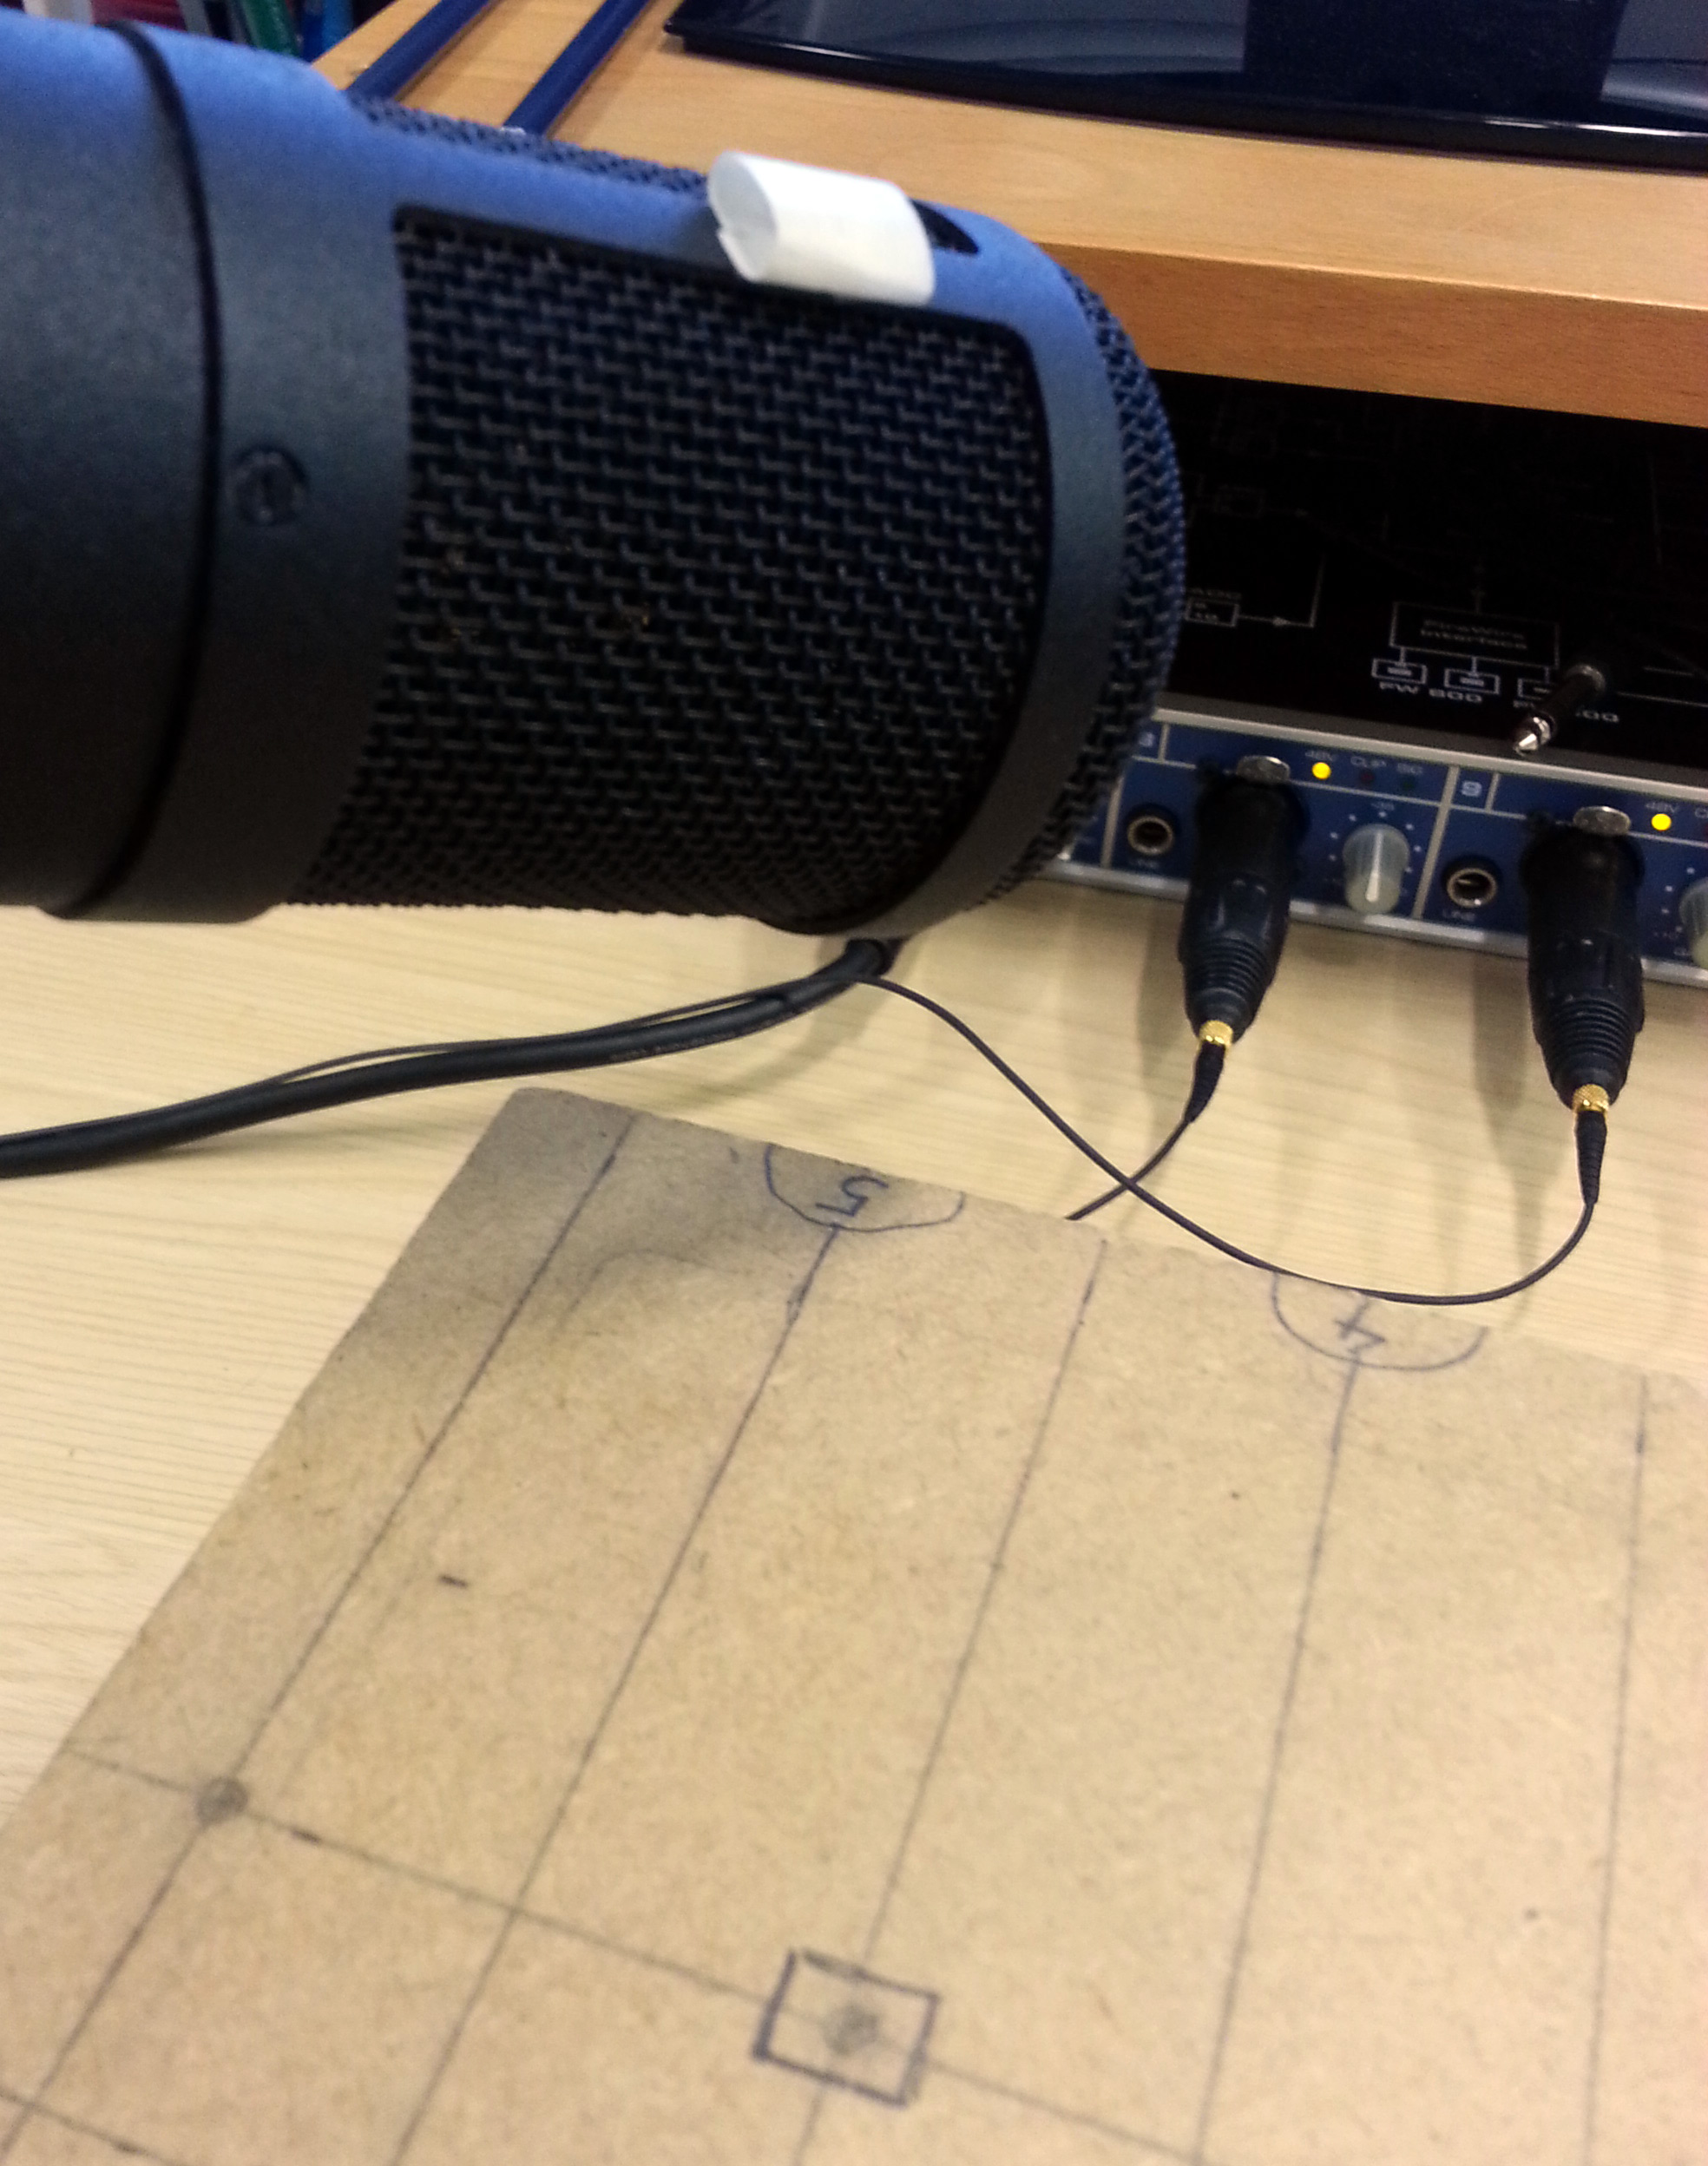
\includegraphics[width=5cm]{mic1}%5
  \caption{Microphone 1 and its placement.}
  \label{fig:mic1}
\end{subfigure}
\caption{Microphones and placements.}
\label{fig:mic123}
\end{figure}

The audio interface used was a RME Firface 800 and can be seen in Figure~\ref{fig:wholesystem}. All data was sampled at 48 kHz at 16 bit.

\section{Pulse alignment test}\label{sec:MultiAPRsystemAligntest}
While the application presented in chapter~\ref{ch:MultichannelAPR} only requires a consistent time alignment between channels, the phase speed calculations of appendix~\ref{ap:SpeedCalc} does rest on the assumption of absolutely aligned channels. To verify this assumption the three microphones were spatially aligned in an open space, as seen in Figure~\ref{fig:micsaligned}, and a sharp pulse, via a forceful hand clap, was applied approximately 4 meters away. The waveform for the pulse onset is presented in Figure~\ref{fig:micsalignedOnset}. Assuming a speed of sound in air at $20\,^{\circ}\mathrm{C}$ $c = 343 \mathrm{m}/\mathrm{s}$. For a signal sampled at 48000 Hz, this gives a ``sample distance'' of about 7 mm.

\begin{figure}
  \centering
  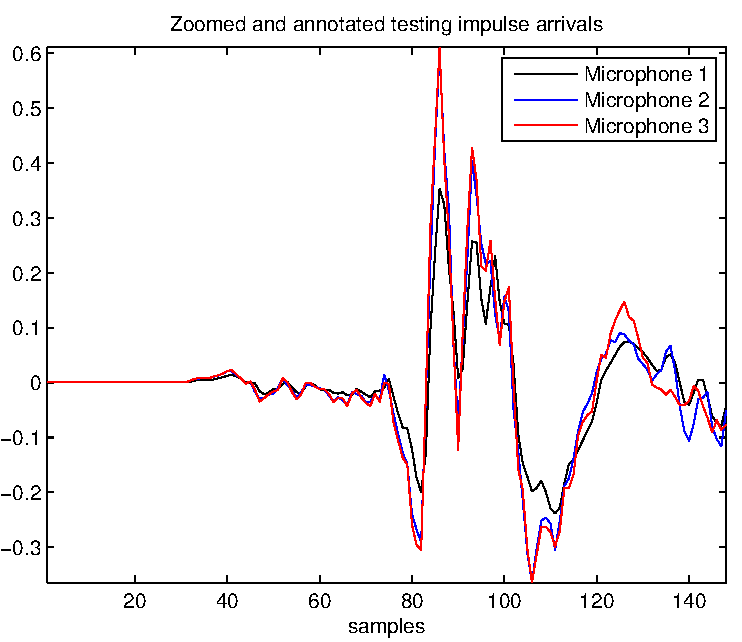
\includegraphics[width=8cm]{alignedTestingImpulses.pdf}%4
\caption{Pulse onset of spatially aligned microphones.}
\label{fig:micsalignedOnset}
\end{figure}

Figure~\ref{fig:micsalignedOnset} shows a feasible perfect alignment given the differences inherent in the microphones. Microphones 2 and 3 are identical with a symmetric placement on the the outside of Microphone 1. The sampled signals appear perfectly aligned.
% ------------------------------------------------------------------------

%%% Local Variables:
%%% mode: latex
%%% TeX-master: "../thesis"
%%% End:
